\section{多项式复杂度}
\label{sec:lpipm-complexity}

单纯形法的换基次数在最坏情形下可以随维数指数增长。内点法能不能给出一个随规模温和增长的迭代次数上界？我们用最容易分析的短步路径跟踪来证明这样的界，再把它翻译成对整个算法运算量的陈述，最后指出这条界和实用规则的距离。

\paragraph{中心路径邻域}
分析的关键是不能让迭代点离路径太远，否则Newton线性化不再可靠。把“靠近路径”写成一个可以检验的条件：

\begin{definition}[中心路径的$\mathcal{N}_2$邻域]
\label{def:lpipm-neighborhood}
对$\theta\in(0,1)$，定义
\begin{equation}
 \mathcal{N}_2(\theta)=\bigl\{(\bm{x},\bm{y},\bm{s})\in\mathcal{F}^{\circ}:\lVert\bm{X}\bm{S}\bm{1}-\mu\bm{1}\rVert_2\leq\theta\mu\bigr\},
 \label{eq:lpipm-n2}
\end{equation}
其中$\mu=\bm{x}^\top\bm{s}/n$。
\end{definition}

条件说的是：把$n$个乘积看成一个向量，它偏离平均值的欧氏长度不超过平均值的$\theta$倍。中心路径上这个偏差是零。这个集合里的每个点都满足$x_is_i\geq(1-\theta)\mu>0$，所以离边界有一定的相对距离。

\paragraph{短步算法}
短步路径跟踪用可行起点，固定取单位步长，让$\mu$每轮按一个很接近$1$的比例减小：
\begin{equation}
 \sigma=1-\frac{0.4}{\sqrt{n}},\qquad\alpha=1,\qquad\theta=0.4.
 \label{eq:lpipm-short-step}
\end{equation}
这里$\sigma$必须和$\sqrt{n}$有关，直观的理由是：$\mu$的相对变化如果太大，乘积向量要移动的距离就会超出邻域。

证明的核心是控制被丢掉的二阶项$\Delta x_i\Delta s_i$。先准备一个关于向量分量乘积的引理。

\begin{lemma}[分量乘积的界]
\label{lem:lpipm-product-bound}
设$\bm{u},\bm{v}\in\mathbb{R}^n$，$\bm{u}^\top\bm{v}\geq0$。记$\bm{U}=\operatorname{diag}(\bm{u})$，$\bm{V}=\operatorname{diag}(\bm{v})$，则
\begin{equation}
 \lVert\bm{U}\bm{V}\bm{1}\rVert_2\leq2^{-3/2}\lVert\bm{u}+\bm{v}\rVert_2^2.
 \label{eq:lpipm-product-bound}
\end{equation}
\end{lemma}

\begin{proof}
把下标分成$P=\{i:u_iv_i\geq0\}$和$Q=\{i:u_iv_i<0\}$。由$\bm{u}^\top\bm{v}\geq0$，
\[
 \sum_{i\in Q}\lvert u_iv_i\rvert\leq\sum_{i\in P}u_iv_i.
\]
对$i\in P$，由$u_iv_i\leq(u_i+v_i)^2/4$，得到
\[
 \sum_{i\in P}u_iv_i\leq\frac14\sum_{i\in P}(u_i+v_i)^2\leq\frac14\lVert\bm{u}+\bm{v}\rVert_2^2.
\]
于是，用向量的$2$范数不超过$1$范数，
\[
 \lVert\bm{U}\bm{V}\bm{1}\rVert_2^2
 \leq\Bigl(\sum_{i\in P}u_iv_i\Bigr)^2+\Bigl(\sum_{i\in Q}\lvert u_iv_i\rvert\Bigr)^2
 \leq2\Bigl(\frac14\lVert\bm{u}+\bm{v}\rVert_2^2\Bigr)^2.
\]
两边开方即得。
\end{proof}

\begin{theorem}[短步路径跟踪的迭代次数]
\label{thm:lpipm-short-step}
设$(\bm{x}^{(0)},\bm{y}^{(0)},\bm{s}^{(0)})\in\mathcal{N}_2(0.4)$，按式~\eqref{eq:lpipm-newton}、\eqref{eq:lpipm-short-step}迭代。则所有迭代点都在$\mathcal{N}_2(0.4)$中，$\mu^{(t+1)}=\sigma\mu^{(t)}$，并且当
\begin{equation}
 T\geq2.5\sqrt{n}\,\log\frac{n\mu^{(0)}}{\varepsilon}
 \label{eq:lpipm-iteration-bound}
\end{equation}
时，$(\bm{x}^{(T)})^\top\bm{s}^{(T)}\leq\varepsilon$。
\end{theorem}

\begin{proof}
记当前点在$\mathcal{N}_2(\theta)$中，$\theta=0.4$，$\mu$为平均互补量。证明分四步。

\emph{第一步，二阶项的大小。}令$\bm{R}=(\bm{X}\bm{S})^{1/2}$，并定义缩放后的方向
\[
 \bm{u}=\bm{R}\bm{X}^{-1}\Delta\bm{x},\qquad\bm{v}=\bm{R}\bm{S}^{-1}\Delta\bm{s}.
\]
当前点可行，所以$\Delta\bm{x}^\top\Delta\bm{s}=0$，从而$\bm{u}^\top\bm{v}=0$。方程组第三行给出
\[
 \bm{u}+\bm{v}=\bm{R}^{-1}\bigl(\bm{S}\Delta\bm{x}+\bm{X}\Delta\bm{s}\bigr)=\bm{R}^{-1}\bigl(\sigma\mu\bm{1}-\bm{X}\bm{S}\bm{1}\bigr).
\]
由引理~\ref{lem:lpipm-product-bound}，注意到$\bm{U}\bm{V}\bm{1}=\Delta\bm{X}\Delta\bm{S}\bm{1}$，以及$\bm{R}^{-2}$的对角元不超过$1/((1-\theta)\mu)$，得到
\[
 \lVert\Delta\bm{X}\Delta\bm{S}\bm{1}\rVert_2\leq\frac{2^{-3/2}}{(1-\theta)\mu}\lVert\sigma\mu\bm{1}-\bm{X}\bm{S}\bm{1}\rVert_2^2.
\]

\emph{第二步，计算右端。}把$\sigma\mu\bm{1}-\bm{X}\bm{S}\bm{1}$写成$(\mu\bm{1}-\bm{X}\bm{S}\bm{1})-(1-\sigma)\mu\bm{1}$。两部分正交，因为$\bm{X}\bm{S}\bm{1}-\mu\bm{1}$的分量之和是$n\mu-n\mu=0$。由勾股定理和邻域条件，
\[
 \lVert\sigma\mu\bm{1}-\bm{X}\bm{S}\bm{1}\rVert_2^2\leq\theta^2\mu^2+(1-\sigma)^2n\mu^2.
\]
代入$\theta=0.4$与$(1-\sigma)^2n=0.16$，结合上一步，得到
\[
 \lVert\Delta\bm{X}\Delta\bm{S}\bm{1}\rVert_2\leq\frac{0.32}{2^{3/2}\times0.6}\,\mu<0.19\,\mu.
\]

\emph{第三步，新点仍在邻域内。}对$\alpha\in[0,1]$，记$\bm{x}(\alpha)=\bm{x}+\alpha\Delta\bm{x}$，$\bm{s}(\alpha)$同理。由第三行，
\[
 x_i(\alpha)s_i(\alpha)=(1-\alpha)x_is_i+\alpha\sigma\mu+\alpha^2\Delta x_i\Delta s_i.
\]
前两项之和不小于$\min\{(1-\theta)\mu,\sigma\mu\}\geq0.6\mu$（$n\geq1$时$\sigma\geq0.6$），第三项的绝对值不超过$0.19\mu$，所以$x_i(\alpha)s_i(\alpha)>0$。乘积从正数出发一直为正，$x_i(\alpha)$和$s_i(\alpha)$就不能变号，因此$\bm{x}^+,\bm{s}^+>\bm{0}$。

$\Delta\bm{x}^\top\Delta\bm{s}=0$说明$\mu^+=\sigma\mu$。$\alpha=1$时，上面的展开给出$x_i^+s_i^+-\sigma\mu=\Delta x_i\Delta s_i$，于是
\[
 \lVert\bm{X}^+\bm{S}^+\bm{1}-\mu^+\bm{1}\rVert_2<0.19\,\mu\leq0.4\,\sigma\mu=\theta\mu^+,
\]
最后一步用到$0.4\sigma\geq0.24$。等式约束由线性性保持，所以新点在$\mathcal{N}_2(0.4)$中。

\emph{第四步，计数。}由上面的结论，$n\mu^{(T)}=n\sigma^T\mu^{(0)}$。利用$\log(1-\beta)\leq-\beta$，只要式~\eqref{eq:lpipm-iteration-bound}成立，就有
\[
 n\mu^{(T)}\leq n\mu^{(0)}\exp\Bigl(-\frac{0.4\,T}{\sqrt{n}}\Bigr)\leq\varepsilon.\qedhere
\]
\end{proof}

这个定理的结构可以这样概括：$\theta$保证Newton步的二阶项足够小，$\sigma$的取法让一步能被邻域容纳，两者的相容性来自$\sqrt{n}$这个因子。由于$(1-\sigma)^2n$要固定，每步减少的比例只能是$1/\sqrt{n}$量级，这就是迭代次数含$\sqrt{n}$的原因。

以贯穿例验证。从中心点$\bm{x}^{(0)}=(6/11,3/11,2/11)^\top$、$y^{(0)}=0$出发，$n=3$，$\sigma=1-0.4/\sqrt{3}\approx0.7691$，起点和前两轮的$\mu$是$0.5455$、$0.4195$、$0.3226$，每轮都乘以$\sigma$。全程相对偏差的最大值约为$0.045$，远小于$0.4$。

取$\varepsilon=10^{-3}$，式~\eqref{eq:lpipm-iteration-bound}给出的上界是
\[
 2.5\sqrt{3}\,\log\frac{18/11}{10^{-3}}\approx32.04,
\]
实际用了$29$轮。短步规则的实际轮数几乎就是理论值，因为$\sigma$是预先固定的。作为对照，第~\ref{sec:lpipm-path-following}节同一个问题用预测—校正把互补量降到$10^{-3}$以下只需$4$轮。

\paragraph{从迭代次数到运算量}
式~\eqref{eq:lpipm-iteration-bound}只计迭代次数。要说“线性规划可以在多项式时间内求解”，还要计入每一轮的代价和数字的长度。整个结论由下面三部分拼成。

第一是每轮的算术运算量：解一个$m\times m$的稠密方程组，需要$O(n^3)$次算术运算（$m\leq n$）。第二是迭代次数中的$\log(n\mu^{(0)}/\varepsilon)$，要说清起点和精度是多少。

第三部分是输入的位长。设数据全部是整数，写出整个问题需要$L$个二进制位，这里$L$至少是$m,n$和各系数位数的总和。可以证明两件事：存在满足定理条件的起点，其$\mu^{(0)}$不超过$2^{O(L)}$，这类起点由第~\ref{sec:lpipm-initial-point}节的嵌入构造给出；只要把间隙降到$2^{-O(L)}$以下，由于有理顶点的分母有界，就可以把近似解精确地修整成最优基。

把这三部分合起来，得到迭代次数$O(\sqrt{n}L)$，算术运算总量$O(n^{3.5}L)$，运算中只需保留$O(L)$位的精度，总的二进制运算量是$L$和$n$的多项式。严格的推导要逐项跟踪精度和起点，篇幅较长，读者可查阅专著\scite{math-bertsimas1997linear}。

这里“多项式”的含义要说准。上面的界依赖$L$，也就是系数的位数，所以这是位模型下的多项式时间，又称弱多项式。是否存在迭代次数只依赖$m,n$、不依赖系数位长的线性规划算法，至今仍是公开问题。内点法的$\log(1/\varepsilon)$项在这里起作用：想要精确解，就需要把精度推到由$L$决定的程度。

\paragraph{理论规则与实用规则}
短步规则的上界最好，实际却很慢：它每轮只减小约$0.4/\sqrt{n}$，从不利用可以走更远的情况。放宽邻域能让步子变大。定义单侧邻域
\begin{equation}
 \mathcal{N}_{-\infty}(\gamma)=\bigl\{(\bm{x},\bm{y},\bm{s})\in\mathcal{F}^{\circ}:x_is_i\geq\gamma\mu,\ i=1,\ldots,n\bigr\},\quad\gamma\in(0,1).
 \label{eq:lpipm-n-inf}
\end{equation}
$\gamma$很小时，几乎只要求每个乘积不要低于平均值太多。图~\ref{fig:lpipm-neighborhoods}(a)是$n=2$时两种邻域在乘积平面上的形状：$\mathcal{N}_2$是窄条，$\mathcal{N}_{-\infty}$几乎占满整个象限。

\begin{BookInlineFigure}
  \centering
  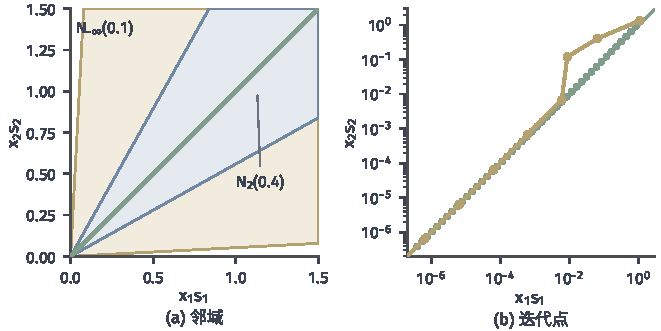
\includegraphics[width=112mm]{figures/05-optimization/01-linear-programming/matplotlib/lpipm-neighborhoods/figure.pdf}
  \caption{$n=2$时中心路径的邻域，横纵轴是两个乘积$x_1s_1,x_2s_2$，绿色对角线是中心路径。(a)蓝色是$\mathcal{N}_2(0.4)$，黄色是$\mathcal{N}_{-\infty}(0.1)$。(b)问题$\min x_1+2x_2$、$x_1+x_2=1$上的迭代点，对数坐标。绿点是短步规则，黄点是$\sigma=0.1$的长步规则，长步规则离路径更远，点数少得多。}
  \label{fig:lpipm-neighborhoods}
\end{BookInlineFigure}

在$\mathcal{N}_{-\infty}(\gamma)$上，每轮取较小的$\sigma$，再沿方向走到将要离开邻域为止，称为长步路径跟踪。它的理论上界是$O(n\log(1/\varepsilon))$，比短步的$O(\sqrt{n}\log(1/\varepsilon))$差，实际表现却远好于短步。

第~\ref{sec:lpipm-path-following}节的预测—校正规则则按式~\eqref{eq:lpipm-sigma-rule}自适应地选$\sigma$，加上二阶校正。按通常的写法，它没有多项式的迭代次数保证，但它是大规模求解器的常用方案。

图~\ref{fig:lpipm-iteration-growth}是随机线性规划上的迭代次数。每个问题都从同一个中心点出发，要求$\mu\leq10^{-6}$。短步规则的轮数紧贴理论值，随$\sqrt{n}$增长，$n=1000$时超过一千轮。长步规则和预测—校正增长得慢得多，$n=1000$时只需$23$轮和$12$轮。

\begin{BookInlineFigure}
  \centering
  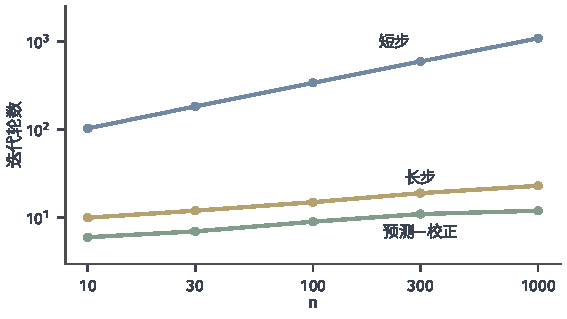
\includegraphics[width=96mm]{figures/05-optimization/01-linear-programming/matplotlib/lpipm-iteration-growth/figure.pdf}
  \caption{随机稠密线性规划上三种规则的迭代轮数，$m=n/2$，对数坐标，起点$\bm{x}=\bm{s}=\bm{1}$是中心点，停止条件$\mu\leq10^{-6}$。蓝线是短步规则，黄线是长步规则（$\sigma=0.1$、$\gamma=10^{-3}$），绿线是预测—校正。每个$n$只运行一个固定种子的实例，用来展示量级而不是平均表现。}
  \label{fig:lpipm-iteration-growth}
\end{BookInlineFigure}

表~\ref{tab:lpipm-rules}把三者放在一起。理论界最好的规则不是实践中最快的规则，这个差距是内点法的一个基本事实。

\begin{BookInlineTable}
  \centering
  \begin{tabular}{@{}llll@{}}
    \toprule
    规则 & 邻域 & 迭代上界 & 实践表现\\
    \midrule
    短步 & $\mathcal{N}_2(0.4)$ & $O(\sqrt{n}\log(1/\varepsilon))$ & 接近理论值，很慢\\
    长步 & $\mathcal{N}_{-\infty}(\gamma)$ & $O(n\log(1/\varepsilon))$ & 轮数少\\
    预测—校正 & 无固定邻域 & 无一般保证 & 通常最少\\
    \bottomrule
  \end{tabular}
  \caption{三种路径跟踪规则的比较。上界针对可行起点；预测—校正指式~\eqref{eq:lpipm-sigma-rule}的常用写法，加上保护措施的变体可以恢复多项式界。}
  \label{tab:lpipm-rules}
\end{BookInlineTable}

\paragraph{历史上的位置}
线性规划的多项式可解性最早不是由内点法确立的。1979年，Khachiyan用椭球法证明了线性规划可以在多项式时间内求解，这个方法每步用一个椭球包住可能的解集，并不断缩小椭球。它在理论上解决了问题，实际计算却很慢。

1984年Karmarkar提出的算法同样具有多项式复杂度，并且在实践中有竞争力，随后的工作发展出本章的原始—对偶路径跟踪。这段历史可以帮助分清两件事：多项式界回答“最坏情形下随规模怎样增长”，实际快慢还取决于常数、结构和实现。
